\documentclass[14pt]{beamer}

\mode<presentation> {
\usetheme{Madrid}

% To remove the navigation symbols from the bottom of all slides uncomment next line
\setbeamertemplate{navigation symbols}{} 
\date{}
\title{}
\author{}

%to get rid of footer entirely uncomment next line
\setbeamertemplate{footline}{}
}


\usepackage{geometry}
\usepackage{multirow}
\usepackage{adjustbox}
\usepackage{multicol}
\setlength{\columnsep}{0.1cm}



\usepackage{tikz}
\usetikzlibrary{shapes,backgrounds}

\usepackage{bbding}
\usepackage{rotating}
\usepackage{xcolor}


%\usepackage{tkz-berge} %cool grid
\usepackage{pgfplots} %pics

\usepackage{graphicx} % Allows including images
\usepackage{booktabs} % Allows the use of \toprule, \midrule and \bottomrule in tables
\usepackage{mathtools}

\newcommand {\DS} [1] {${\displaystyle #1}$}
\newcommand {\R}{\mathbb{R}}
\newcommand {\Z}{\mathbb{Z}}
\newcommand {\N}{\mathbb{N}}
\newcommand{\e}{\varepsilon}

\newcommand{\p}{\pause}

% simple environrment for enumerate, easier to read
\setbeamertemplate{enumerate items}[default]

%%%%%%%%%%%%%%%%%%%%%%

% to use colours easily
\definecolor{miverde}{rgb}{0.7, .5, 0.7}
\newcommand{\azul}[1]{{\color{blue} #1}}
\newcommand{\rojo}[1]{{\color{red} #1}}
\newcommand{\verde}[1]{{\color{miverde} #1}}
 
% box in red and blue in math and outside of math
\newcommand{\cajar}[1]{\boxed{\mbox{\rojo{ #1}}}}
\newcommand{\majar}[1]{\boxed{\rojo{ #1}}}
\newcommand{\cajab}[1]{\boxed{\mbox{\azul{ #1}}}}
\newcommand{\majab}[1]{\boxed{\azul{ #1}}}
 
\newcommand{\setsize}[1]{\fontsize{#1}{#1}\selectfont} %allows you to change the font size. The default size of this document is 14. To change the font size of the whole slide, place this at the beginning of the slide. To change the size of only a portion of the text to size 12, you can do the following { \setsize{12} Your text. }.

\setbeamerfont{frametitle}{size=\setsize{15}}
\setbeamerfont{block title}{size=\setsize{14}}

\newcommand{\smallerfont}{\setsize{13}} %place this at the beginning of a slide to set the font size of the entire slide to 13.

%===========================
% SPECIAL PREAMBLE JUST FOR TODAY
%===========================

 \newcommand{\chords}{
	\draw (0,0) circle [radius=2.5] ;
	\draw[red, thick] (-2.5,0) to (1.5, 2)  ;
	\draw[red, thick] (-2.5,0) to (0, -2.5)  ;
	\draw[red, thick] (-2.5,0) to (2.3, -0.97)  ;
	\draw[red, thick] (2.3,-0.97) to (1.5, 2)  ;
	\draw[red, thick] (0,-2.5) to (1.5, 2)  ;
	\draw[red, thick] (2.3,-0.97) to (0, -2.5)  ;
	\draw[fill] (1.5,2) circle [radius=0.1] ;
	\draw[fill] (0,-2.5) circle [radius=0.1] ;
	\draw[fill] (-2.5,0) circle [radius=0.1] ;
	\draw[fill] (2.3,-0.97) circle [radius=0.1] ;
}

\usepackage{makecell}


\setbeamertemplate{enumerate items}{(\Alph{enumi})}


%===================================================
\begin{document}
%===================================================

%----------------------------------------------------------------------------------------
%	CLASS QUESTIONS
%----------------------------------------------------------------------------------------

%------------------------------
\begin{frame}[t]
\frametitle{Welcome to MAT137 - Calculus with proofs!}


\begin{itemize}
	\item Class begins 10 minutes after the hour
	\item Your instructor is Professor Jason Siefken
	\item Course website:  \cajab{https://q.utoronto.ca}
		
	\vfill
	\item  {\bf Before next class:}
		\begin{itemize} \normalsize
			\item {\bf Watch videos 1.1, 1.2, 1.3 }
		\end{itemize}
	\vfill
\end{itemize}

\end{frame}
%------------------------------
%-----------------------------
\begin{frame} 
\begin{center}
	{\Large
		How do students do in MAT137?
		\vfill
		\pause
		It depends on \\ how many problem sets they submit.
		\vfill
	}
\end{center}

\end{frame}
%-------------------------
\begin{frame}
	\includegraphics[width=\textwidth]{137_1819_GradesVsPS}
\end{frame}
%------------------------------
\begin{frame}{Quick exercise}
\smallerfont
 \p

Take 45 seconds to look over the following list of pairs of words, \\ but {\bf do not write anything down}.

\p

\begin{table}[h]
\centering
\begin{tabular}{@{}ll@{}}
\toprule
bread/b\underline{\ \ }tter & ocean/breeze \\
leaf/tree & music/l\underline{\ \ }rics\\
sweet/sour & sh\underline{\ \ }e/sock\\
phone/bo\underline{\ \ }k & movie/actress \\
chi\underline{\ \ }s/salsa & gasoline/engine \\
high school/college & pen\underline{\ \ }il/paper\\
river/b\underline{\ \ }at & turkey/stuffing \\
fruit/vegetable & be\underline{\ \ }r/wine\\
computer/chip & television/rad\underline{\ \ }o\\
l\underline{\ \ }nch/dinner & chair/couch \\
\bottomrule
\end{tabular}
\end{table}

\end{frame}
% ----------------------------------------------------------------------  
\begin{frame}{What do you remember?}

\p

\begin{itemize}
	\item[] Write down as many pairs of words as you can.
	\item[] You do \emph{not} need to remember which letters were missing or which
		column they were in.
\end{itemize}

\end{frame}
% ----------------------------------------------------------------------  
\begin{frame}[t]{What did you remember?}
\smallerfont

\p

Mark each pair you remembered as ``A" or ``B"

\

\begin{table}[h]
\centering
\begin{tabular}{@{}ll@{}}
\toprule
\makecell[c]{A} & \makecell[c]{B}  \\
\midrule
ocean/breeze & bread/b\underline{\ \ }tter\\
leaf/tree & music/l\underline{\ \ }rics\\
sweet/sour & sh\underline{\ \ }e/sock\\
movie/actress & phone/bo\underline{\ \ }k\\
gasoline/engine & chi\underline{\ \ }s/salsa\\
high school/college & pen\underline{\ \ }il/paper\\
turkey/stuffing & river/b\underline{\ \ }at\\
fruit/vegetable & be\underline{\ \ }r/wine\\
computer/chip & television/rad\underline{\ \ }o\\
chair/couch & l\underline{\ \ }nch/dinner\\
\bottomrule
\end{tabular}
\caption{Word list from \alert{The Talent Code} (by Daniel Coyle).}
\end{table}

\end{frame}
%-----------------------------
%-----------------------------
\begin{frame}
\frametitle{A warm-up problem}

\begin{itemize}
	\item<2-> Pick 4 points at random on a circle\\  (without any symmetry).
	\item<3->  Join every pair of points.
	\item<4->  In how many regions is the circle divided?
\end{itemize}
\begin{center}
\begin{tikzpicture}
\only<2->{		\draw (0,0) circle [radius=2.5] ;  }
\only<3->{		\draw[red, thick] (-2.5,0) to (1.5, 2)  ; }
\only<3->{		\draw[red, thick] (-2.5,0) to (0, -2.5)  ; }
\only<3->{		\draw[red, thick] (-2.5,0) to (2.3, -0.97)  ; }
\only<3->{		\draw[red, thick] (2.3,-0.97) to (1.5, 2)  ; }
\only<3->{		\draw[red, thick] (0,-2.5) to (1.5, 2)  ; }
\only<3->{		\draw[red, thick] (2.3,-0.97) to (0, -2.5)  ; }
\only<2->{		\draw[fill] (1.5,2) circle [radius=0.1] ; }
\only<2->{		\draw[fill] (0,-2.5) circle [radius=0.1] ; }
\only<2->{		\draw[fill] (-2.5,0) circle [radius=0.1] ; }
\only<2->{		\draw[fill] (2.3,-0.97) circle [radius=0.1] ; }
\end{tikzpicture}
\end{center}	

\end{frame}
%-----------------------------
%------------------------------
\begin{frame}
\smallerfont
\frametitle{Fire}
Which of the following statements are equivalent to the statement,
	\begin{center}
	\emph{``No two students in this class are not on fire.''}
	\end{center}

Which are equivalent to its negation?  

\vfill

	\begin{enumerate}
		\item ``All student in this class, except at most one, are on fire.''
		\item ``Two students in this class are on fire.''
		\item ``For any pair of students in this class, one of them is on fire.''
		\item ``At least two students in this class are not on fire.''
		\item ``If I choose two students in this class and one of them is not on fire, then the other one is on fire.''
	\end{enumerate}

\vfill

\end{frame}
%-----------------------------
\end{document}
%-----------------------------
%-----------------------------
%-----------------------------









